\documentclass[UTF8, xcolor=table]{beamer}
\usepackage[BoldFont,SlantFont]{xeCJK}
\setCJKmainfont[BoldFont={Adobe Heiti Std},ItalicFont={Adobe Kaiti Std}]{AdobeSongStd-Light}
% \setCJKmainfont[BoldFont={Adobe Heiti Std},ItalicFont={Adobe Kaiti Std}]{SimSum} %Windows先编译使用这个字体

\usepackage{latexsym,amssymb,amsmath,amsbsy,amsopn,amstext,xcolor,multicol}
\usepackage{graphicx,wrapfig,fancybox}
\usepackage{pgf,pgfarrows,pgfnodes,pgfautomata,pgfheaps,pgfshade}
\usepackage{thubeamer}
\usepackage[backend=bibtex,sorting=none]{biblatex} % [参考文献格式](https://www.sharelatex.com/blog/2013/07/31/getting-started-with-biblatex.html) %mac IEEE not found
\usepackage{array}
\usepackage{bm}
\usepackage{caption}
\RequirePackage[font=footnotesize]{subcaption}
\usepackage{multirow}
\usepackage{booktabs}
\usepackage{tikz}
\usepackage{tikzscale}
\usepackage{animate}

\defbibheading{bibliography}[\bibname]{} %avoid printbibliography 自动生成目录
\addbibresource{../main.bib}
\setbeamertemplate{bibliography item}[text] 

\usepackage{boxedminipage} %for: bvh border
\def\fourgraphicswidth{0.35} %0.3\textwidth

\usepackage{algorithm} %%format of the algorithm
\usepackage{algpseudocode}
\floatname{algorithm}{算法}
\renewcommand{\algorithmicrequire}{\textbf{输入:}} % Use Input in the format of Algorithm
\renewcommand{\algorithmicensure}{\textbf{输出:}} % UseOutput in the format of Algorithm
\algrenewcommand{\algorithmiccomment}[1]{ $//$ #1}

\usepackage{listings}
\renewcommand\lstlistingname{代码}
\renewcommand\lstlistlistingname{代码}

\lstset{framexleftmargin=1.4em,
        xleftmargin=1.8em,
        basicstyle=\ttfamily\small,
        %frame=shadowbox, numberstyle=\tiny, breaklines=true,
        frame=single,
        numberstyle=\tiny, breaklines=true,
        keywordstyle=\color{blue!70}\bfseries,
        %commentstyle=\color{red!50!green!50!blue!50},
        rulesepcolor=\color{red!20!green!20!blue!20},
        numbers=none,fontadjust=true}
\lstdefinelanguage{shader}{morekeywords={uniform, layout, uniform, vec2, vec3, vec4, in, out, gl_Position, dot, flat, int ,float, gl_VertexID, xyz, w, x, y, z, location, version, sampler2DRect, bgr, gl_FragData, texture2DRect, gl_TexCoord,for,xy},morecomment=[l]{//}}

\begin{document}

\setbeamerfont{footnote}{size=\tiny}
\setbeamerfont{caption}{size=\scriptsize}
\setbeamertemplate{caption}[numbered]
\setbeamerfont{subsection in toc}{size=\footnotesize}
\renewcommand*{\bibfont}{\footnotesize}

\graphicspath{{../}}

\title[融合长短记忆神经网络与卷积特征学习的图像语义分割]{中山大学本科毕业论文演示文稿非正式模版}
\author[陈冠英]{}%{(申请中山大学工学学士学位论文答辩报告)\\ \vskip 20pt 学~~~~~~生:陈~冠~英}
\institute[中山大学~电子信息与工程学院~\&~自动化]{}%{\small \vskip 38pt 电子信息与工程学院~自动化}
\date{} %{\small \vskip -17pt二〇一六年五月}

%% make title %%
\frame{
	\titlepage
	\vspace{-23mm}
	\begin{figure}[h]
		\centering
		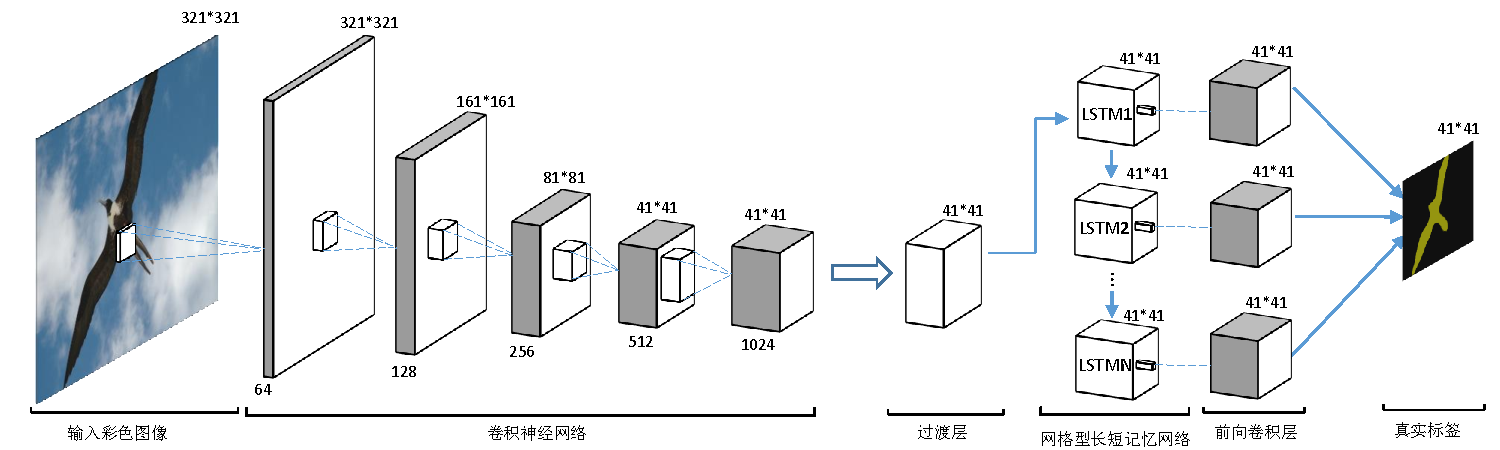
\includegraphics[width=\textwidth]{image/illustration/networkstructure.pdf}
	\end{figure}
}

\frame {
	\frametitle{目录}
	%\begin{multicols}{2}
	\tableofcontents[sections={<1-7>}]
}

\chapter{绪论}
本章介绍了无线传感网的结构及其应用领域。分析规模化无线传感网的特点,对规模化传感网数据认证的需求和面临的挑战进行了分析。概述了本文的研究内容,并对文章的组织结构予以说明。
\section{本文研究背景和意义}
无线传感器网络(Wireless Sensor Networks,无线传感网)是一种特殊组织结构的移动自组网\upcite{c:sensor},在环境监测、工业控制、资源监控、智能家居、医疗保健和军事等各种领域都有广泛应用,有非常重要的地位和作用。
随着无线传感网技术的不断发展,很多应用进入了日常生活中,物联网技术也将成为未来发展的重要方向。
无线传感网的各种技术发展紧跟具体的应用需求,随着各种应用场景需要的安全性越来越高,安全问题也成为了阻碍无线传感网大规模发展的一个制约。

大范围监测在环境监测和军事侦察等诸多关系国家社会重大安全的领域都具有重要的地位和作用。在环境监测领域,往往面临范围野外受限甚至恶劣条件,在海洋等资源监测领域,水声通信等基础技术还不是很完善, 在军事侦察对抗领域更是要应对破坏攻击情况,传统的大范围实时监测机制和系统都难以得到有效部署,使用无线传感技术成为了最好的解决方案。规模化无线传感网因此应运而生,而且为满足大范围监测的需要,无线传感网的规模越来越大。

规模化无线传感网面临的安全威胁更多,攻击的影响更大,而且由于传感器节点的特点,传统的安全机制和协议无法直接适用于无线传感网,使得安全问题更加凸显。因此针对规模化无线传感网安全机制的研究成为了热门研究方向。

\subsection{无线传感网概述}
\subsubsection{无线传感网结构}
无线传感器节点被部署在目标监测区域,大量的传感器节点通过无线广播的方式,以一定的算法自组织成为一个多跳的无线网络。如图~\ref{fig:cluster}所示,是一个典型无线传感网的结构\upcite{c:cluster},由三部分组成:监测区域的传感器节点、与外部网络连接的网关或基站、远程数据中心。在监测区域的传感器节点一般通过算法组成若干的簇,每个簇通过簇头节点与其他簇或者基站通信,这样的方案节约了节点的能量。簇内节点收集到监测数据以后通过簇头节点的整合,形成报文通过一定的路径发送给基站,基站进一步通过外部网络设备,如互联网、卫星等将监测数据传输到远程数据中心。

\begin{figure}[htbp]
  \centering
  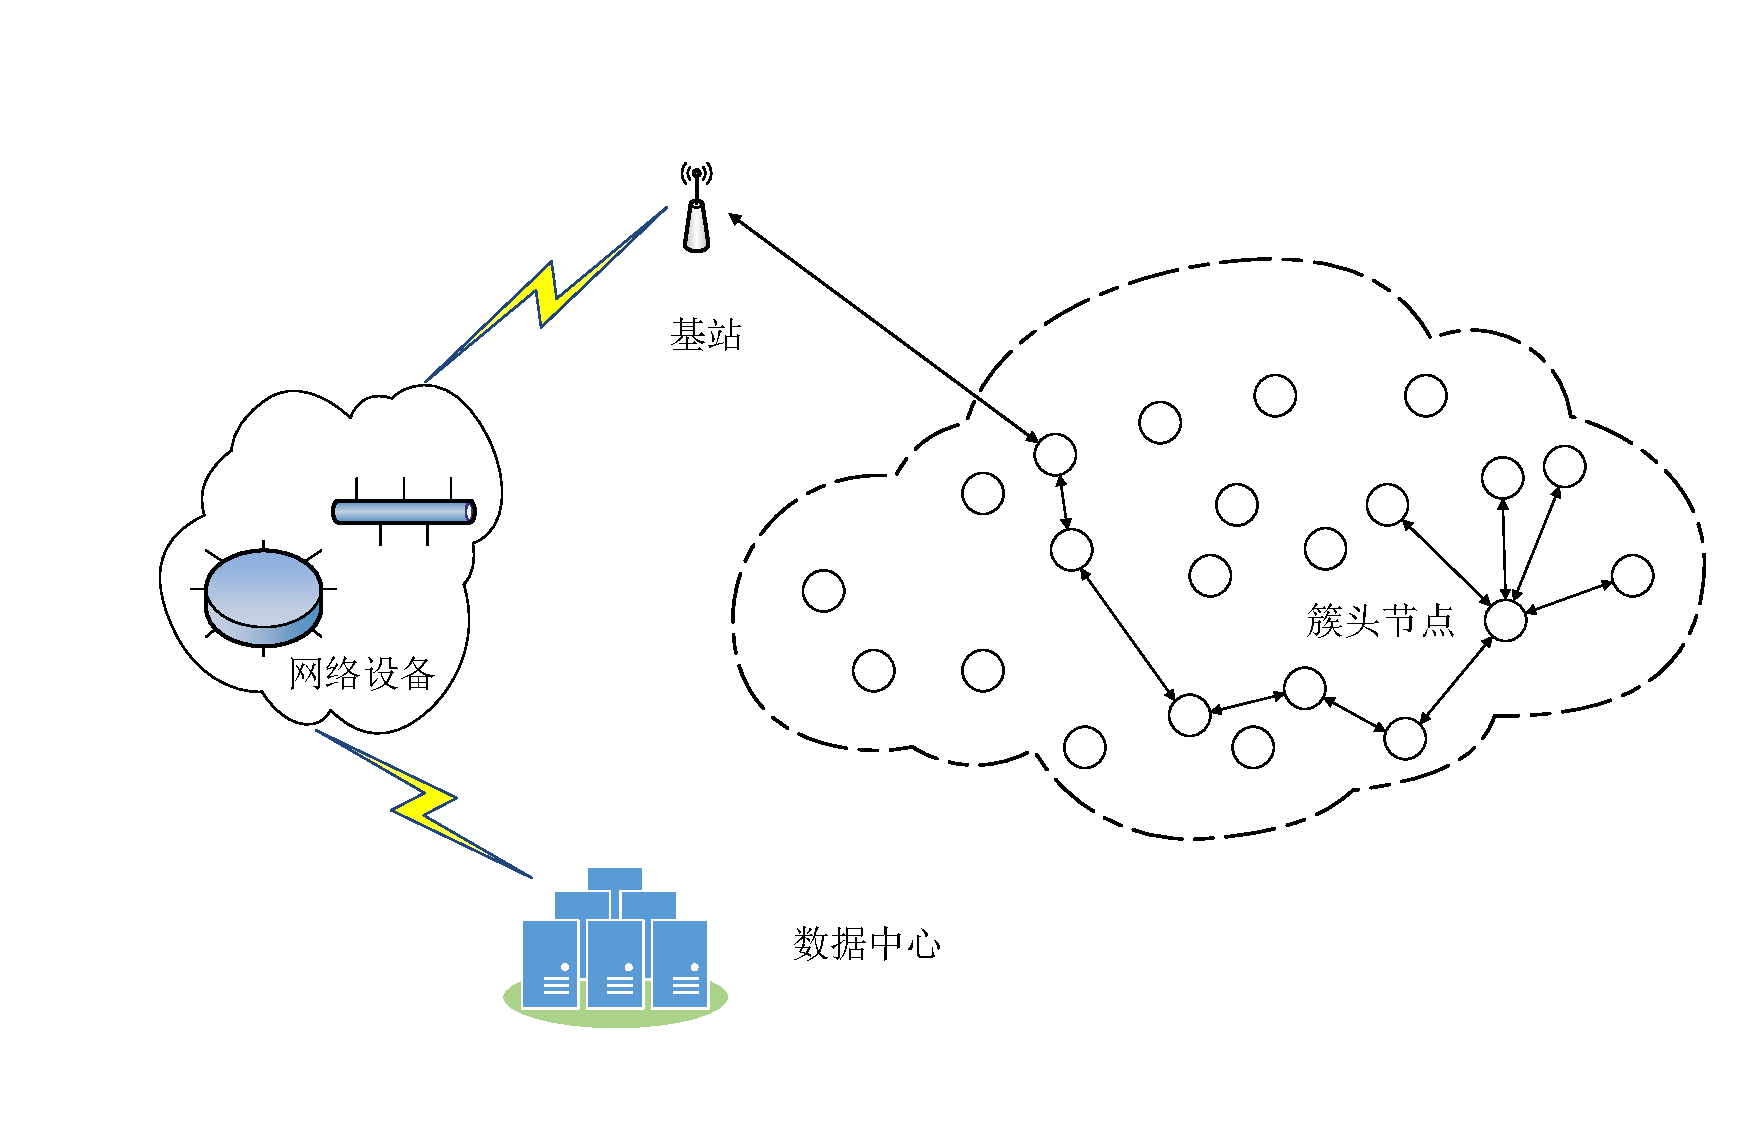
\includegraphics[width=5in]{cluster}
  \caption{无线传感网系统结构}
  \label{fig:cluster}
\end{figure}


无线传感网中,基站的计算和存储能力都比较强,
基站的功能可以是一个数据处理中心,向网络广播控制信息,从监测区域获取数据。
也可以是一个网络网关,负责数据向远程数据中心的传输。

\subsubsection{无线传感器节点结构}
传感器节点是无线传感网的基本组成单元,负责数据采集、发送等基本功能。
无线传感器节点一般仅具有很小的存储空间,较弱的计算能力,因此单个节点无法完成复杂的感知任务,需要大量的节点协同工作。

随着电子技术的发展,无线传感器节点的性能也有了很大的提升,如Crossbow公司研发的TelosB,CPU频率为8MHz,有10KB的RAM,使用2.4GHz无线电,能达到250Kbps数据传输,使用两节AAA电池(5号电池)供电。国产传感器节点典型的有美新的MEMSIC无线模块,工作频率可选433 MHz、868-915MHz或2.4GHz,拥有5年电池寿命,支持10-100米的发射范围,拥有19.2kbps-240kbps的数据传输速率。

\begin{figure}[htbp]
  \centering
  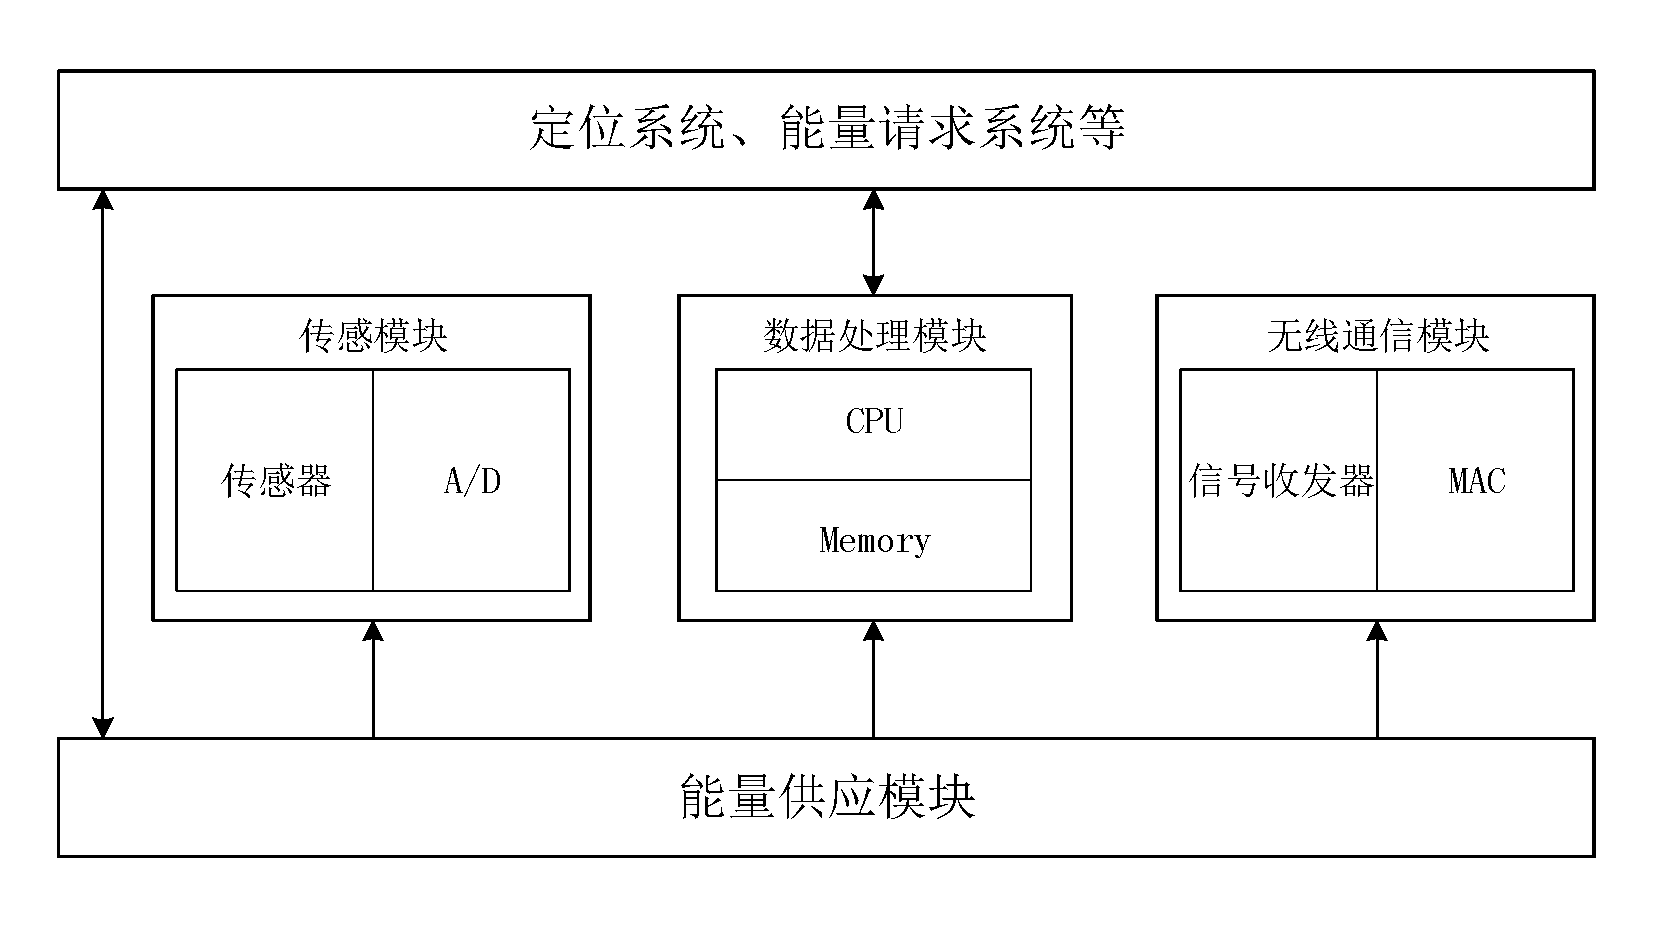
\includegraphics[width=5in]{node}
  \caption{无线传感网节点结构}
  \label{fig:node}
\end{figure}

这些传感器节点的设计原理基本相同,主要包括4个模块:传感模块、数据处理模块、无线通信模块和能量供应模块。
如图~\ref{fig:node}所示,是一个典型的无线传感器节点的结构图。传感模块主要负责从感知区域通过传感器获取数据,并将数据转化为适合进行网络传输的数字信号;数据处理模块主要包括处理和存储功能,负责控制传感器节点的运行,对传感模块获取的数据进行处理和存储,数据报文的整合与认证都是由数据处理模块完成,一般该模块需要嵌入式系统的支持,如UC Berkeley的开源嵌入式系统TinyOS\upcite{c:tinyos}等;无线通信模块负责与其他传感器节点或基站之间的通信,传感器节点一般使用内置天线进行数据收发;能量供应模块负责给其他模块供应能量,大部分传感器节点使用微型电池作为电源,因此能量非常有限。传感器节点中还包括一些负责定位、同步等功能的部件。

\subsubsection{无线传感网协议结构}

\begin{figure}[htbp]
  \centering
  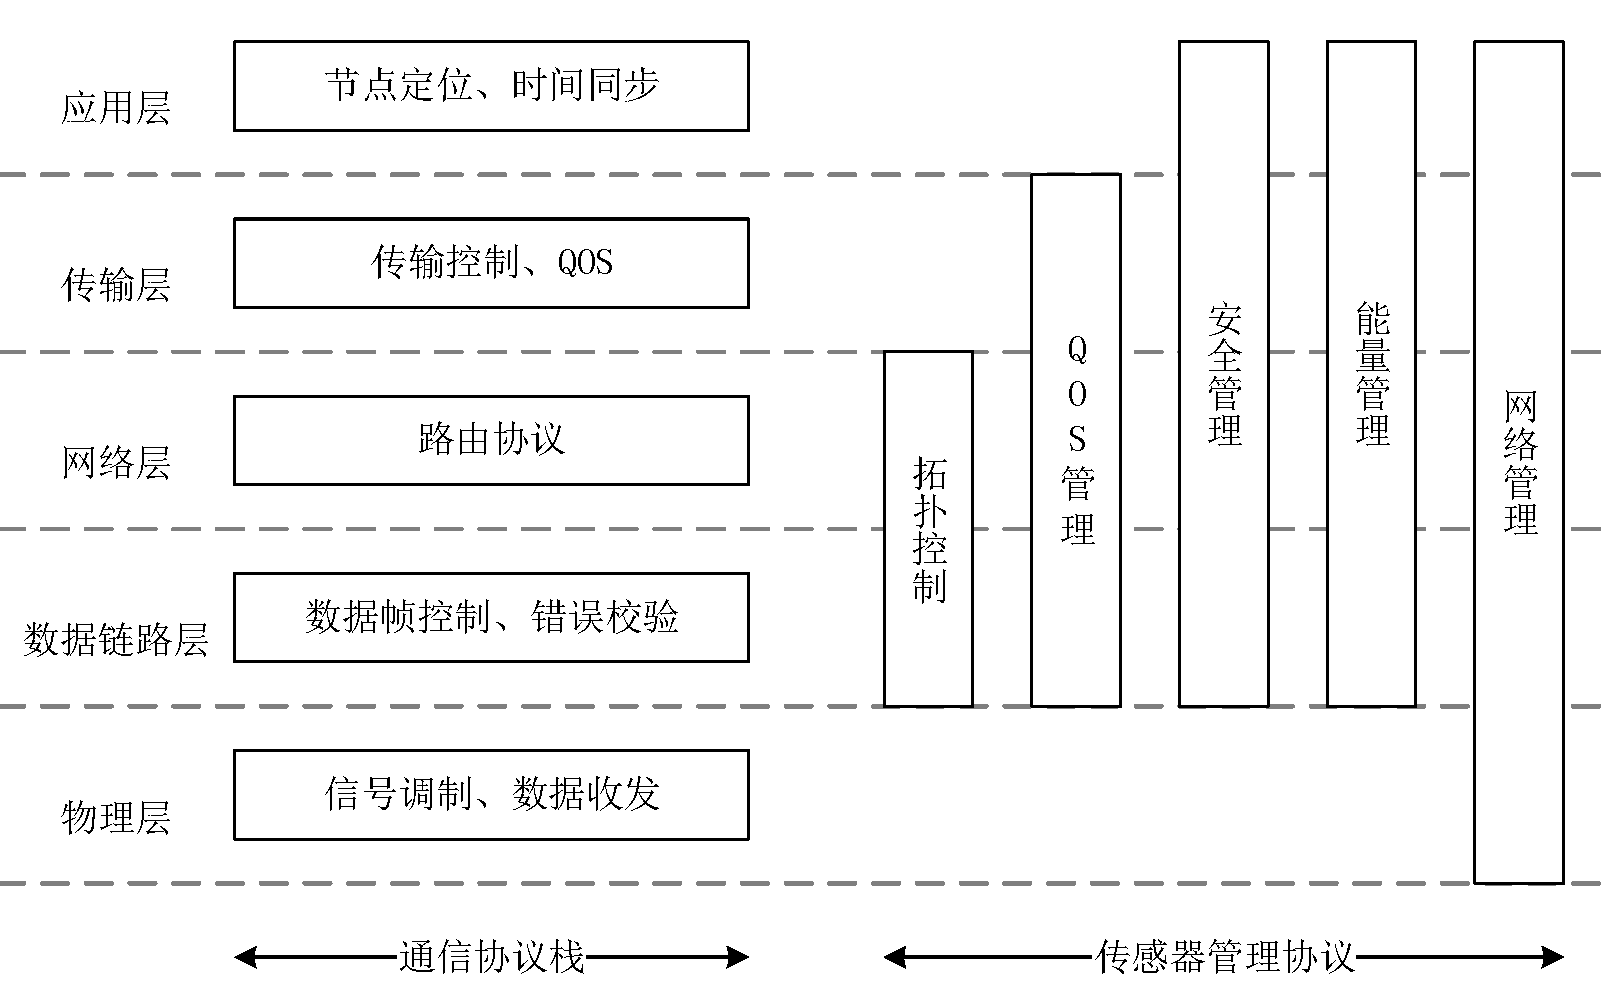
\includegraphics[width=5in]{construction}
  \caption{无线传感网协议结构}
  \label{fig:construction}
\end{figure}
无线传感网的通信协议栈和相关网络管理技术是当前的主要研究内容,协议结构如图~\ref{fig:construction}所示。
因为无线传感网是面向特定需求的网络,因此针对不同的部署环境,不同的网络部署结构,要对通信协议栈进行优化,使能量消耗、抗节点损耗、抗攻击能力等适应传感网的应用需求。

类似于OSI网络模型,无线传感网的通信协议栈由物理层、数据链路层、网络层、传输层、应用层组成:

物理层:物理层是通信协议栈的最底层,主要功能是将数据调制成适合传输的数字信号,通过无线电、红外灯无线介质完成传感器节点的数据收发。

数据链路层:数据链路层负责装配数据帧,对数据帧进行MAC校验,进行差错控制,向网络层提供透明可靠的数据传输服务。

网络层:主要负责无线传感网中的路由功能,将数据通过有效路径传送到目标节点,向传输层提供端对端的数据传输服务。

传输层:传输层负责数据报文的传送和控制,为应用层提供可靠的传输服务,对网络进行流量控制,进行服务质量控制(QOS)。

应用层:直接为应用提供服务,提供相应的应用协议和服务接口。

传感网管理协议提供了拓扑管理、QOS管理、安全管理、能量管理和网络管理等功能,实现对无线传感网以及各个节点的监控和管理。
\subsubsection{无线传感网的应用前景}
分布式传感网在军事中的应用是无线传感网的雏形,随着电子技术的不断发展,传感器节点的性能不断提升,无线传感网各种协议的完善和发展,使无线传感网在环境监测、军事侦察、智能家居、智能公路等各个领域得到了大量的应用,其应用前景十分广泛。

\begin{compactitem}
  \item 环境监测:无线传感网能完成大范围监测的任务,在自然数据采集中发挥重要作用,尤其是海洋监测传感网和内陆水文传感网等应用领域。如Li 等人将无线传感网部署在水产养殖水域,对水环境数据进行检测\upcite{c:water}。
  \item 军事侦察:由于无线传感网具有自组网、部署简单、容许节点失效等特点,适合部署在危险的敌对区域,完成军事侦察、战场环境监测等任务,因而在军事领域有很大应用前景,是现代化电子战的重要战略武器。如美国海军将开发的自主分布式DADS(Deployable Autonomous Distributed System)用于沿海广大海域的警戒、反潜和反水雷\upcite{c:DADS}。
  \item 智能家居:智能家居是通过无线传感器将房间中的各种家电等设备连接起来,实现家居环境的监测以及远程控制,构建出智能的居住环境\upcite{c:homes}。
  \item 智能公路:通过部署在公路上的无线传感器节点以及车载传感器节点,共同组成智能公路传感网络,对交通状况实现自动监测,引导车流等,实现自动化的公路交通管理。
\end{compactitem}



\subsection{规模化无线传感网数据认证}
\subsubsection{规模化无线传感网的特点}
规模化无线传感网是为满足大范围监测的需要而产生的,如国内著名的绿野千传项目,在浙江省天目山建立的大规林业监测传感网,部署的自组织传感网节点超过2000个,网络中传输路径跳数超过 20 跳
\upcite{c:lvye}。
规模化无线传感网具有如下的特点:
\begin{enumerate}\setlength{\itemsep}{-\itemsep}
  \item 节点数量大,覆盖面积广,节点失效较为频繁,网络拓扑结构相对不稳定。
  \item 一般部署于恶劣区域,甚至是敌对攻击区域,恶意攻击的频度增加。
  \item 节点的计算和存储能力更为受限,网络的能量较为敏感,对机制的轻量化要求更突出。
\end{enumerate}

\subsubsection{规模化无线传感网的数据认证需求}
无线传感网中的认证包括身份认证和数据认证。身份认证是对网络中节点的合法身份的一种判定机制,是数据认证的基础。无线传感网数据认证主要包括两个方面:
\begin{compactitem}
  \item 数据来源合法性,主要以身份认证为基础,通过数据报文中的认证机制判定数据报文的来源的合法性。
  \item 数据完整性,通过数据认证的机制,确保节点收到的数据报文没有被非法进行篡改。
\end{compactitem}

在环境监测等领域,规模化传感网每天都会产生海量的感知数据。在军事侦察领域,随着侦察区域的扩大,侦察精度的提高,传感网感知的数据量飞速增长。尤其在实时监测场景,数据量大、传输实时性要求高,无线传感器节点的性能限制使得规模化传感网实现可靠传输具有非常的难度,合适的数据认证机制可以为其提供有力支持。在无线传感网中数据泄露、错误数据甚至虚假数据会对网络的安全造成重大影响。尤其在重要战略场景或军事场景,还要考虑破坏攻击的可能,因此数据认证更为安全攸关。
\subsubsection{规模化无线传感网数据认证面临的挑战}

复杂环境下数据高安全性要求对数据认证提出的挑战。实时监测传感网通常部署环境恶劣,而且缺乏基础设施的建设,由于自然环境和主动攻击等对节点的破坏,使节点的失效率很高,网络拓扑结构动态变化,数据传输质量不够稳定,而且存在突发大故障潜因,需要在容灾抗毁前提下进行数据认证,确保传输的安全性。

端对端传输为数据认证提出的挑战。完全依靠广播等数据传输机制,在规模化无线传感网中,传输效率过低,消耗的节点能量和通信资源过大,而且容易受到泛洪攻击的影响。有效利用规模化传感网中端对端数据传输,能够有效的保证传输效率。在端对端传输中,由于多跳传输的原因,当路径中出现妥协节点时,整条路径容易被攻破,从而造成数据传输被攻击,因而在多路径端对端的数据传输中,有效利用数据认证机制加强路径上的安全保障是安全传输的关键。

轻量级认证机制及其实现技术为数据认证提出的挑战。规模化无线传感网传输的数据量大,要求处理快捷。在节点资源能力受限,通信能耗受限的前提下,需要计算、存储、通信都轻量级的水平,保障网络安全、传输可靠性、高效性和数据可信,具有很大难度。传统的的认证机制使用的密码算法复杂度未达到轻量级,不适合规模化传感网网络资源受限的特点,我们需要设计适合实时性较高的规模无线传感网达到轻量级算法。

攻击对抗对数据认证提出的挑战。无线传感网一般部署在恶劣环境中,而且具有自组网络的多跳性、无中心性和自组织性等特征,致使其通信协议栈的各个层级都容易遭受到各种形式的攻击,我们需要设计能够适应有限节点能量,有限计算能力的数据认证算法,对抗各种攻击,保证无线传感网传输数据的来源合法性和完整性。

\section{本文研究内容}
本文根据规模化无线传感网的安全需求以及其特点,针对其数据认证关键技术展开研究,使用多节点联合的技术思路研究数据认证模型和机制,并设计实现了关键算法。
主要工作如下:

\begin{enumerate}\setlength{\itemsep}{-\itemsep}
  \item 提出了多跳长路径上多节点联合数据认证的模型,设计了多跳长路径上多节点联合数据认证协议,并设计了路径上节点关系的维护算法,对协议的安全性能进行了分析评价。
  \item 针对多跳长路径上多写点联合数据认证协议的不足,对算法进行了优化,提出了多路径抗节点失效机制和动态步长多节点联合数据认证机制,并对优化方案的安全性能进行了分析评价。
  \item 围绕多跳长路径多节点联合数据认证机制的需求,对密钥分配方案进行了深入研究,提出了基于单向hash链的密钥分配方案,并对认证中的MAC进行了研究,提出了适应数据认证机制需求的MAC码。
\end{enumerate}


\section{本文组织结构}
本文一共分为七章。

第一章\quad 绪论,介绍了课题的选题背景,描述了无线传感网的特点,介绍了无线传感网的相关安全技术,列出了本文的主要研究内容和本文组织结构。

第二章\quad 相关研究概述,本章首先对无线传感网的安全技术进行了概述,然后重点对数据认证和密钥分配两种安全技术进行了论述。

第三章\quad 多跳长路径上多节点联合数据认证,本章提出了无线传感网中多跳长路径多节点联合的数据认证模型,及其设计目标。
重点介绍了关键算法与协议的设计实现,对多节点联合数据认证机制的安全性能进行了分析评价。

第四章\quad 数据认证方案优化,本章针对多跳长路径上多节点联合数据认证进行了优化,提出了多路径抗节点失效和动态步长多节点联合数据认证两个优化方案,并对它们的安全性能进行了分析评价。

第五章\quad 密钥分配与MAC设计,本章对多节点联合数据认证中的密钥分配方案以及使用的MAC的设计进行了介绍,提出了基于单向hash链的密钥分配方案,以及适应多节点联合数据认证的MAC码。

第六章\quad 仿真实验与结果分析,本章在仿真平台上对多跳长路径多节点联合数据认证机制,以及其优化方案进行了仿真实验,对它们的安全性能结果进行了评价。

第七章\quad 总结与展望,本章对全文的工作做了总结,指出了数据认证机制现阶段的不足以及未来研究中需要研究及完善的地方。


\chapter{中华人民共和国}
\label{cha:china}

\section{图的例子}
\label{sec:other}

在第~\ref{cha:intro} 章中我们学习了贝叶斯公式~(\ref{equ:chap1:bayes}),这里我们复
习一下:
\begin{equation}
\label{equ:chap2:bayes}
p(y|\mathbf{x}) = \frac{p(\mathbf{x},y)}{p(\mathbf{x})}=
\frac{p(\mathbf{x}|y)p(y)}{p(\mathbf{x})}
\end{equation}

\subsection{绘图}
\label{sec:draw}

本模板不再预先装载任何绘图包(如 \textsf{pstricks,pgf} 等),完全由你自己来决定。
个人觉得 \textsf{pgf} 不错,不依赖于 Postscript。此外还有很多针对 \LaTeX{} 的
 GUI 作图工具,如 XFig(jFig), WinFig, Tpx, Ipe, Dia, Inkscape, LaTeXPiX,
jPicEdt, jaxdraw 等等。

\subsection{插图}
\label{sec:graphs}
关于子图形的使用细节请参看 \textsf{subcaption} 的说明文档。

\subsection{一个图形}
\label{sec:onefig}
一般图形都是处在浮动环境中。之所以称为浮动是指最终排版效果图形的位置不一定与源文
件中的位置对应\footnote{This is not a bug, but a feature of
\LaTeX!},这也是刚使 用 \LaTeX{}
同学可能遇到的问题。如果要强制固定浮动图形的位置,请使用
\textsf{float} 宏包, 它提供了 \texttt{[H]}
参数,比如图~\ref{fig:heythere}。
\begin{figure}[H] % use float package if you want it here
  \centering
  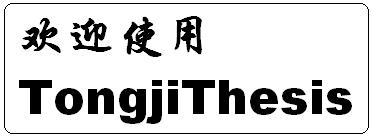
\includegraphics[height=2cm]{hello.jpg}
  \caption{插个图插个图}
  \label{fig:heythere}
\end{figure}

大学之道,在明明德,在亲民,在止于至善。知止而后有定;定而后能静;静而后能安;安
而后能虑;虑而后能得。物有本末,事有终始。知所先后,则近道矣。古之欲明明德于天
下者,先治其国;欲治其国者,先齐其家;欲齐其家者,先修其身;欲修其身者,先正其心;
欲正其心者,先诚其意;欲诚其意者,先致其知;致知在格物。物格而后知至;知至而后
意诚;意诚而后心正;心正而后身 修;身修而后家齐;家齐而后国治;国治而后天下
平。自天子以至于庶人,壹是皆以修身为本。其本乱而未治者 否矣。其所厚者薄,而其所
薄者厚,未之有也!

\hfill \pozhehao《大学》


\subsection{简单子图}
\label{sec:multifig}

如果多个图形相互独立,并不共用一个图形计数器,那么用 \verb|minipage| 或者
\verb|parbox| 就可以。否则,请参看图~\ref{fig:big1},它包含两个小图,分别是图~\ref{fig:subfig1}
和图~\ref{fig:subfig2}。推荐使用 \verb|\subcaption|,不要再用\verb|\subfloat|,\verb|\subfigure| 和 \verb|\subtable|了。
\begin{figure} %[h]
  \centering%
  \subcaptionbox{第一个小图形\label{fig:subfig1}}{%    
    
\includegraphics[height=2cm]{tongji-fig-logo.png}}\hspace{4em}%
  \subcaptionbox{第二个小图形。如果标题很长的话,它会自动换行,这个 caption 就是这样的例子\label{fig:subfig2}}{%    
    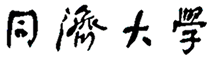
\includegraphics[height=2cm]{tongji-text-logo.png}}
  \caption{包含子图形的大图形}
  \label{fig:big1}
\end{figure}

古之学者必有师。师者,所以传道受业解惑也。人非生而知之者,孰能无惑?惑而不从师,
其为惑也,终不解矣。生乎吾前,其闻道也固先乎吾,吾从而师之;生乎吾後,其闻道也亦
先乎吾,吾从而师之。吾师道也,夫庸知其年之先後生於吾乎!是故无贵无贱无长无少,道
之所存,师之所存也。

嗟乎!师道之不传也久矣,欲人之无惑也难矣。古之圣人,其出人也远矣,犹且从师而问焉;
今之众人,其下圣人也亦远矣,而耻学於师。是故圣益圣,愚益愚。圣人之所以为圣,愚
人之所以为愚,其皆出於此乎?爱其子,择师而教之,於其身也,则耻师焉,惑焉。彼童子
之师,授之书而习其句读者,非吾所谓传其道、解其惑者也。句读之不知,惑之不解,或师
焉,或不焉,小学而大遗,吾未见其明也。巫医、乐师、百工之人不耻相师,  士大夫之族
曰“师”曰“弟子”之云者,则群聚而笑之。问之,则曰:彼与彼年相若也,道相似也,位
卑则足羞,官盛则近谀。呜呼!师道之不复,可知矣。巫医、乐师、百工之人。吾子不齿,
今其智乃反不能及,其可怪也欤!圣人无常师。孔子师郯子、苌子、师襄、老聃。郯子之徒,
其贤不及孔子。孔子曰:“三人行,必有我师。”是故弟子不必不如师,师不必贤於弟子。
闻道有先後,术业有专攻,如是而已。

\subsection{复杂子图要注意遮挡}
使用子图的方法如图~\ref{fig:chap2:zitu}所示,使用\texttt{subcaptionbox}环境设置每一个子图,注意\texttt{subcaptionbox}其后需要有括号,以及子图换行时需要使用\texttt{vskip},以免下一排子图会对上一排子图的图名造成遮挡。
\begin{figure}[htbp]
\centering
  \subcaptionbox{第一个小图形}{\label{fig:chap1:zitu:a}
  
\includegraphics[width=5cm]{tongji-fig-logo}\hskip2cm}
  \subcaptionbox{第二个小图形}{\label{fig:chap1:zitu:b}
  
\includegraphics[width=5cm]{tongji-fig-logo}}
\vskip0.5cm
  \subcaptionbox{第三个小图形}{\label{fig:chap1:zitu:c}
  
\includegraphics[width=5cm]{tongji-fig-logo}\hskip2cm}
  \subcaptionbox{第四个小图形}{\label{fig:chap1:zitu:d}
  
\includegraphics[width=5cm]{tongji-fig-logo}}
\caption{多子图用\texttt{subcaptionbox}}\label{fig:chap2:zitu}
\end{figure}


\subsection{多个图形独立}
如果要把编号的两个图形并排,那么小页就非常有用了,如图~\ref{fig:parallel2}:
\begin{figure}
\begin{minipage}{0.48\textwidth}
  \centering
  
\includegraphics[height=2cm]{tongji-whole-logo.png}
  \caption{并排第一个图}
  \label{fig:parallel1}
\end{minipage}\hfill
\begin{minipage}{0.48\textwidth}
  \centering
  
\includegraphics[height=2cm]{tongji-whole-logo.png}
  \caption{并排第二个图}
  \label{fig:parallel2}
\end{minipage}
\end{figure}


李氏子蟠,年十七,好古文、六艺,经传皆通习之,不拘於时,学於余。余嘉其能行古
道,作师说以贻之。

\hfill \pozhehao 韩愈(唐)


\subsection{插图大原则}
同志们,如果遇到问题一定要会搜索,要么看别人的问答,要么看宏包的文档,希望你不要成为重度伸手党。
一点微小的工作,谢谢大家。

\section{插入pdf格式图片的问题}
\label{sec:problem}
在\LaTeX{}中插入高清图片一般有两种方式:1)插入~eps~矢量图,2)插入~pdf~格式图片。在模板测试过程中遇到一个插入
~pdf~格式图片的问题。

问题描述

插入~pdf~格式的图,有时采用~XeLaTeX~编译后,插图被翻转~90~度。有时却不会出现该问题。问题图片如图~\ref{rotatedBode}~所示。
\begin{figure}[H] 
  \centering
  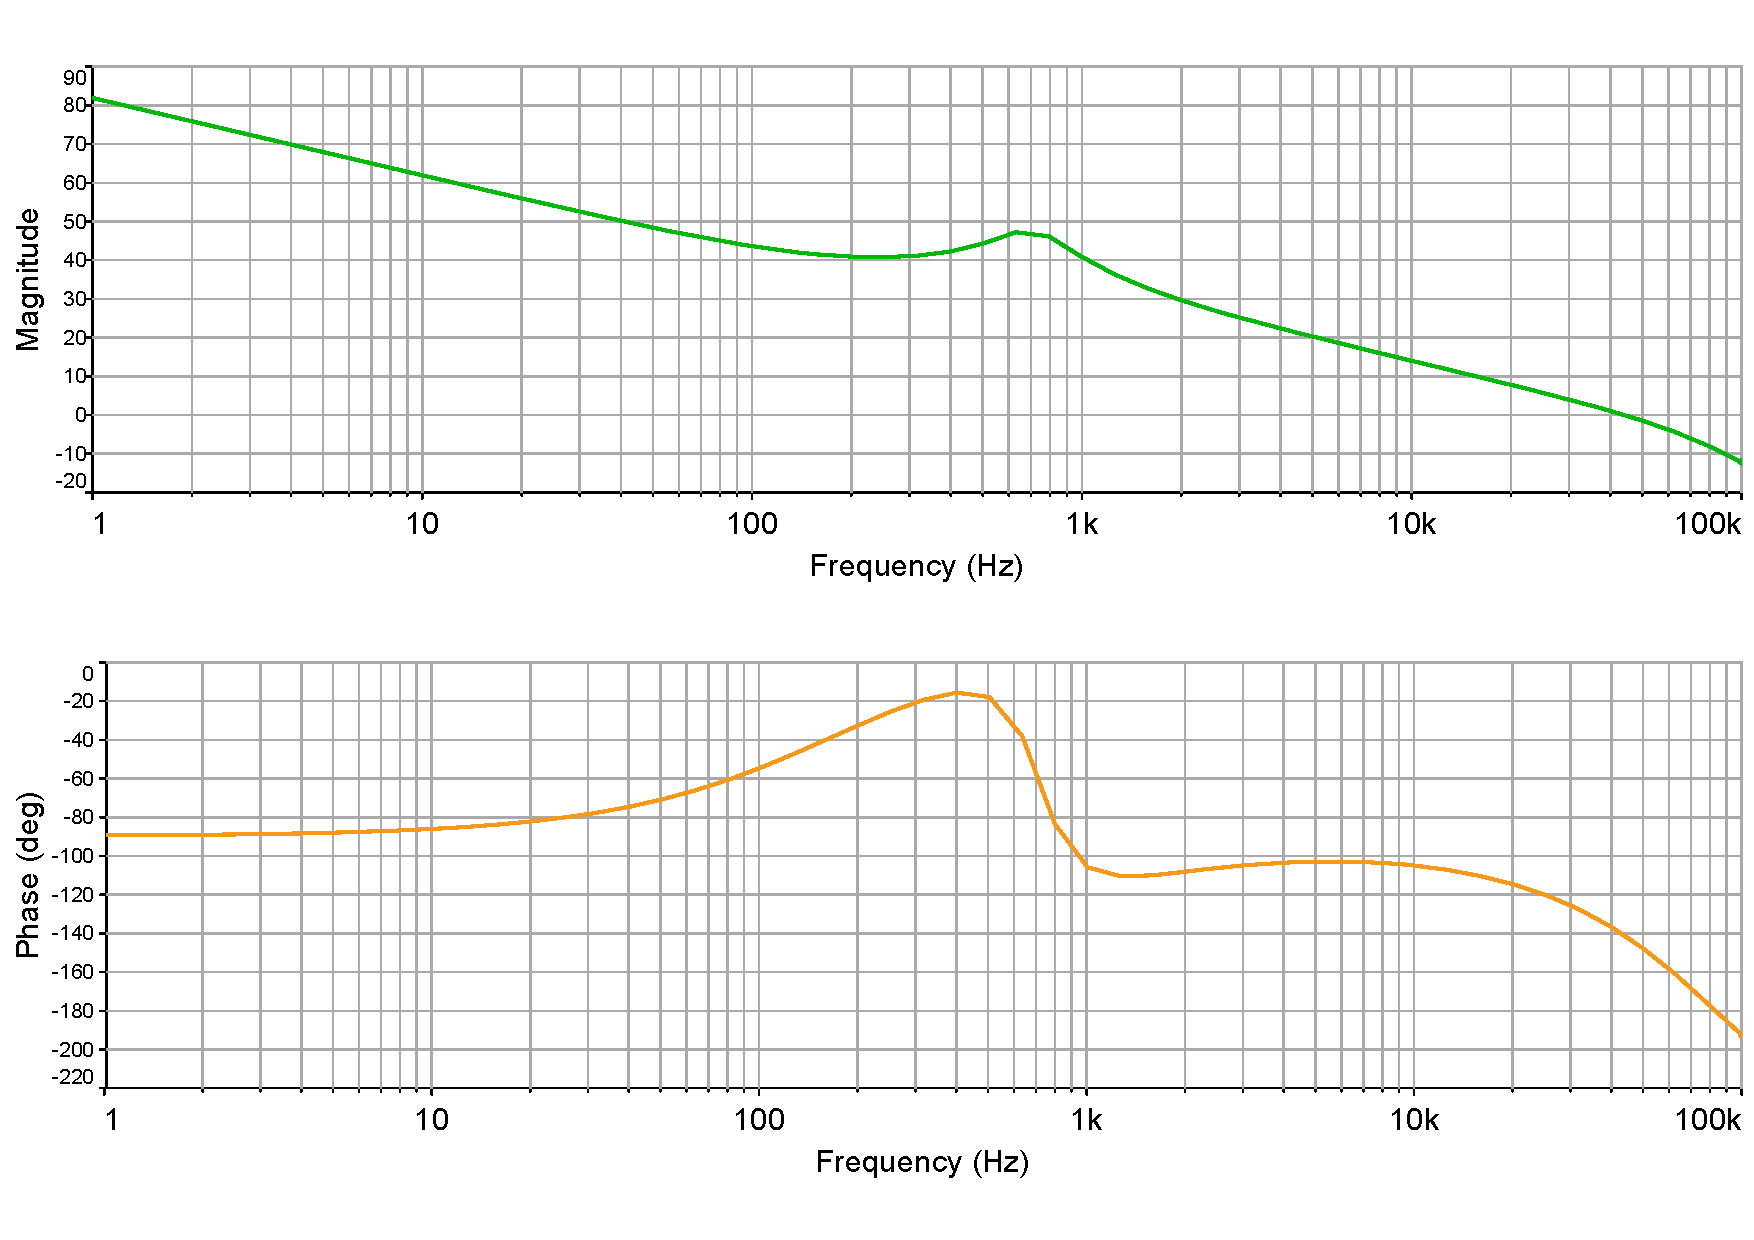
\includegraphics[width=12cm]{BodeGraph.pdf}
  \caption{被自动翻转的bode图}
  \label{rotatedBode}
\end{figure}

问题原因

同一幅图片,XeLaTeX~编译出现图片翻转,而~pdfLaTeX~编译,输出正常。
原因可能是出现在~XeLaTeX~编译过程中会将有些~pdf~文件自身多余的旋转命令编译出来。

问题解决方法

第一种方法(抄自刘海洋大牛的方案):
使用命令\\ \texttt{pdfcrop foo.pdf foo-new.pdf},当然,新文件名可以和旧文件名相同。 这个方法的好处就是 pdfcrop 是texlive自带的,我装的是texlive2017,因此自带了。

第二种方法:采用GhostScript软件消除多余的旋转命令。
\begin{enumerate}
    \item 下载安装~GhostScript~软件,官网为\url{https://www.ghostscript.com/download/gsdnld.html/}
        
    \item 将安装后的bin文件夹地址加入用户环境变量,在我电脑上为~\verb|D:|\verb|\Program Files|\verb|\gs|\verb|\gs9.22|\verb|\bin|
	
    \item cmd~命令行进入想转换图片所在文件夹,执行命令\\gswin32c -sDEVICE=pdfwrite -o newname.pdf  previousname.pdf
              得到一个去除多余旋转命令的~newname.pdf~文件。

    \item 在\LaTeX{}中插入该~pdf~文件,XeLaTeX~编译。
\end{enumerate}

处理之后的图片如图~\ref{Bode}~所示。
\begin{figure}[H] 
  \centering
  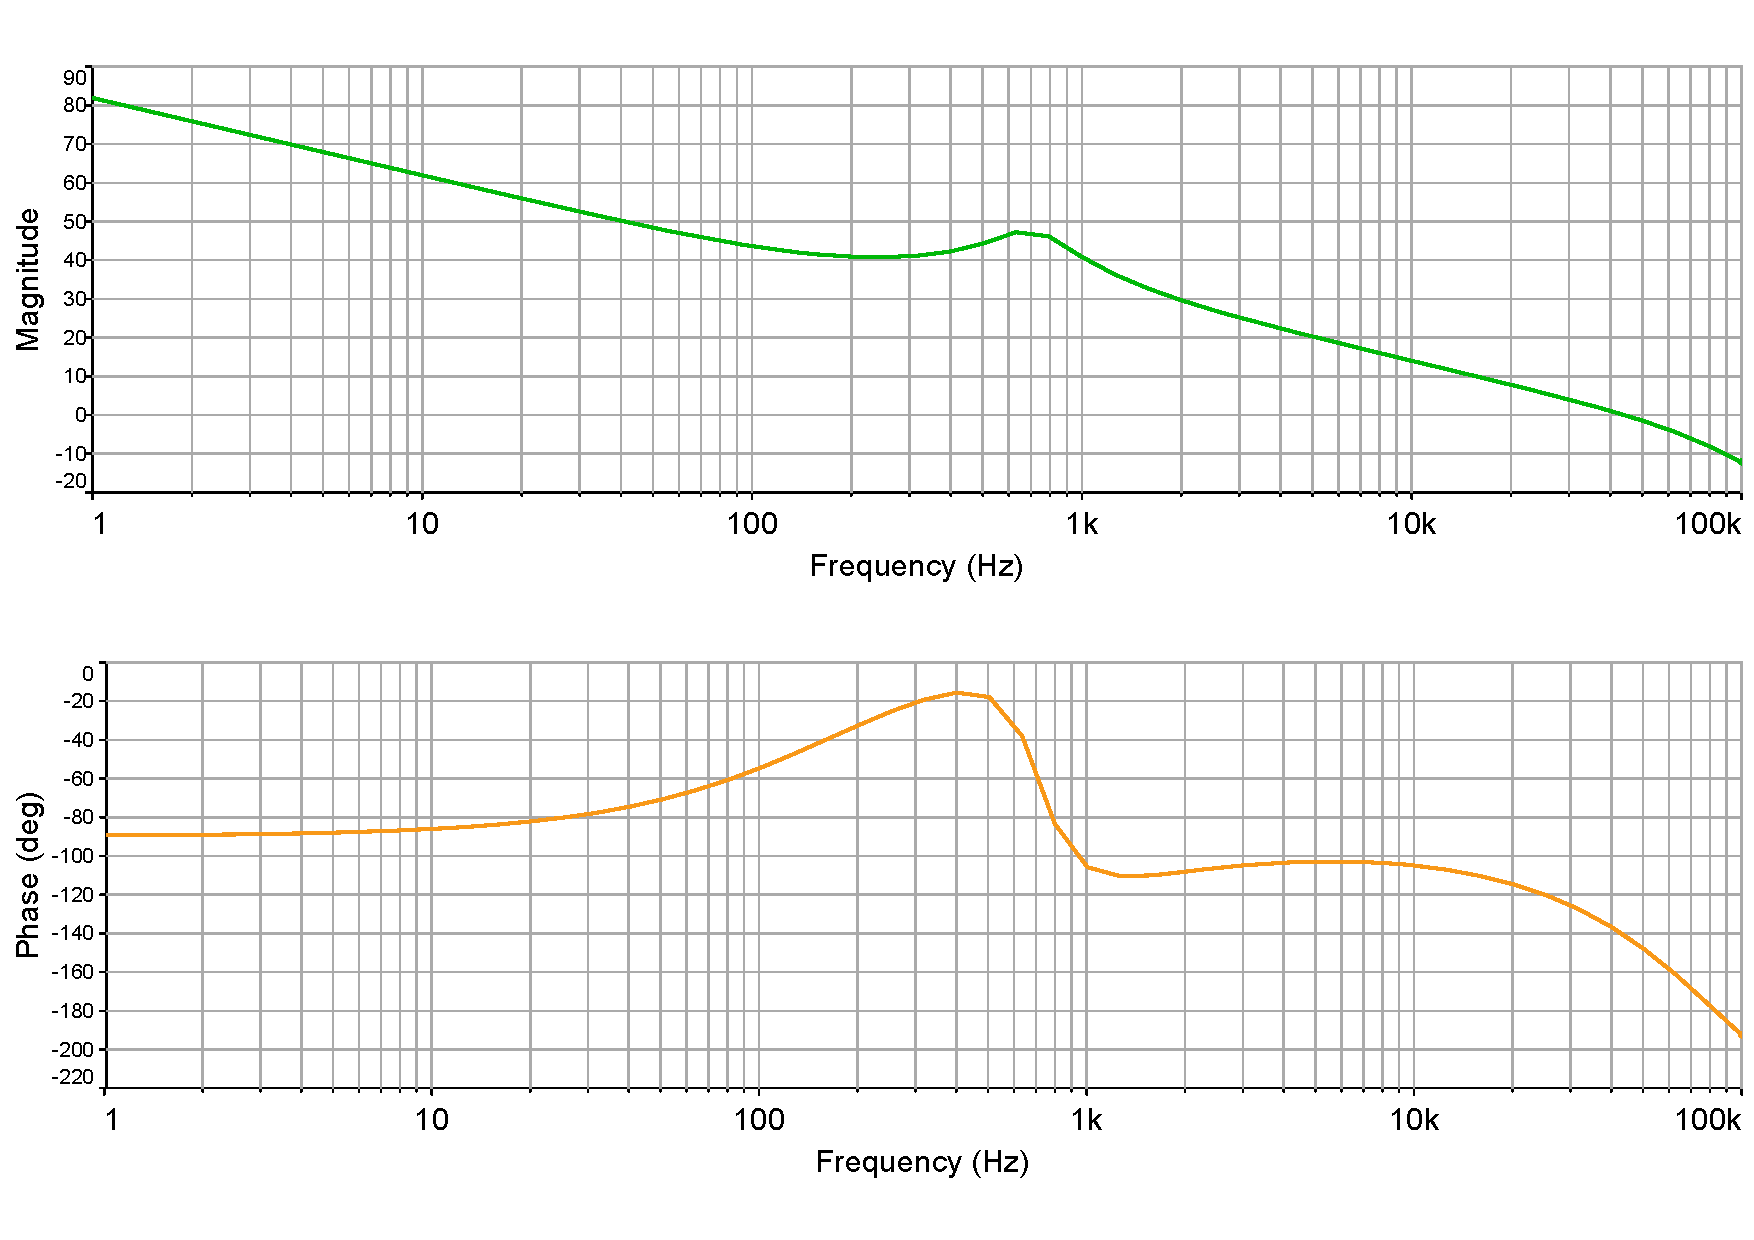
\includegraphics[width=12cm]{Bode.pdf}
  \caption{处理后的bode图}
  \label{Bode}
\end{figure}






\section{网络模型结构}
\subsection*{网络模型结构}
\frame{
  \frametitle{网络整体结构}
	\begin{figure}[h]
		\centering
		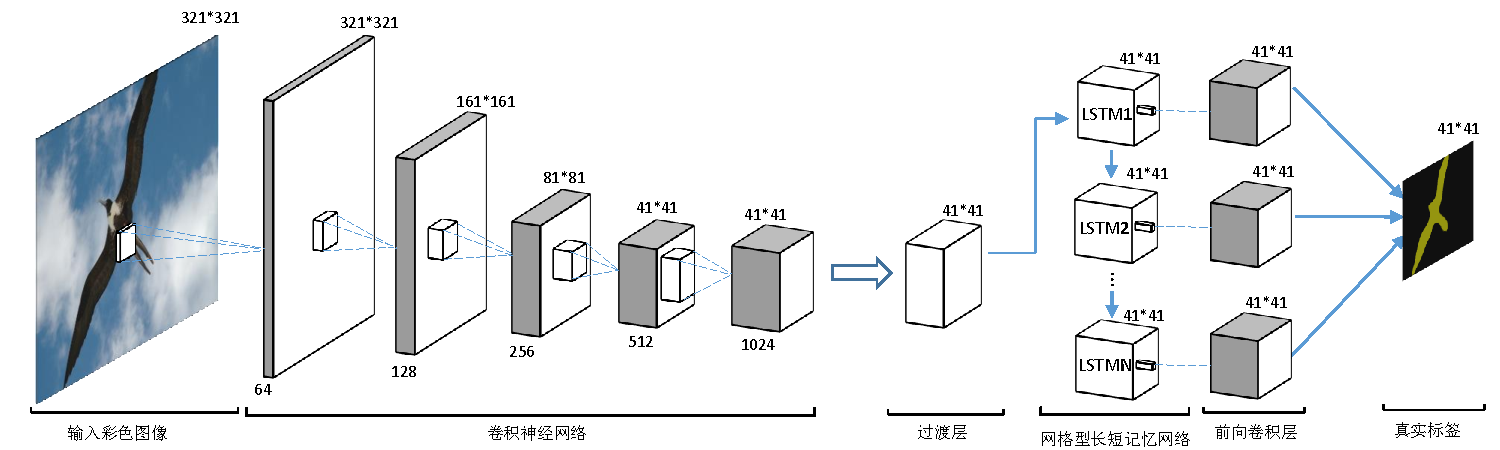
\includegraphics[width=0.9\textwidth,height=0.28\textwidth]{image/illustration/networkstructure.pdf}
		\caption{网络整体结构图}
		\label{fig:networkstructure}
	\end{figure}
	\vspace{-1em}
	\small
	\begin{block}{}
	\begin{itemize}
		\item  四个组成部分:\textbf{卷积网络部分},过渡层,\textbf{网格型长短记忆网络部分},前向卷积层
		\item 核心思想:在卷积网络后堆叠多层网格型长短记忆层
	\end{itemize}
	\end{block}
}
\frame{
	\frametitle{卷积网络部分}
	\vspace{-1em}
	\footnotesize
	\begin{block}{}
	\begin{itemize}
		\item 基于$VGG_{16}$模型\footnote{Simonyan \& Zissermanet, Very deep Convolutional Networks For Large-scale Image Recognition, ICLR 2015}, 含有16层卷积层
		\item 使用了“孔算法”,在不损失精度的情况下将模型参数减少了 6.5 倍\footnote{Chen et al, DeepLab-LargeFOV, ICLR 2015}
	\end{itemize}
	\end{block}
	\vspace{-1em}
	\begin{figure}[h]
		\centering
		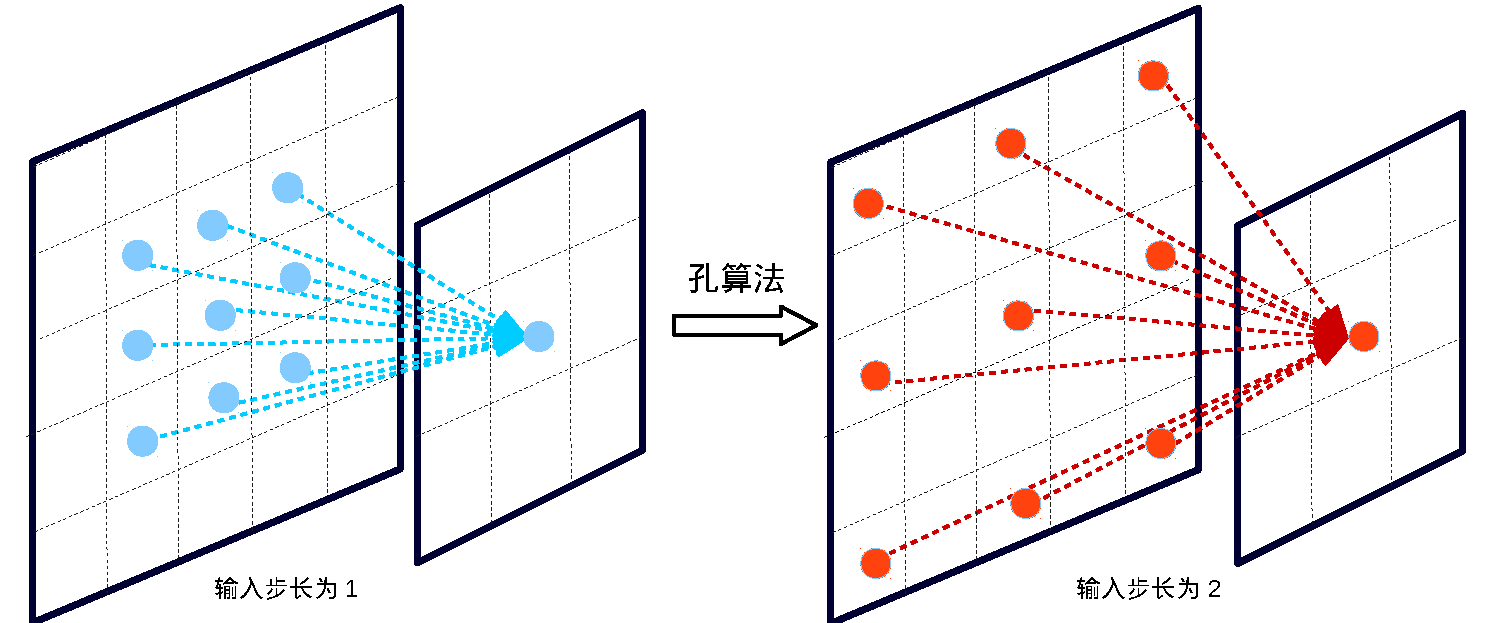
\includegraphics[width=0.7\textwidth]{image/illustration/hole.pdf}
		\caption{"孔算法"示意图}
	\end{figure}
}

\frame{
\frametitle{网格型长短记忆网络部分}
	\vspace{-1em}
    \begin{columns}%[onlytextwidth]
        \begin{column}{0.6\textwidth}
        \vspace{0.2em}
		\begin{figure}
			\centering
			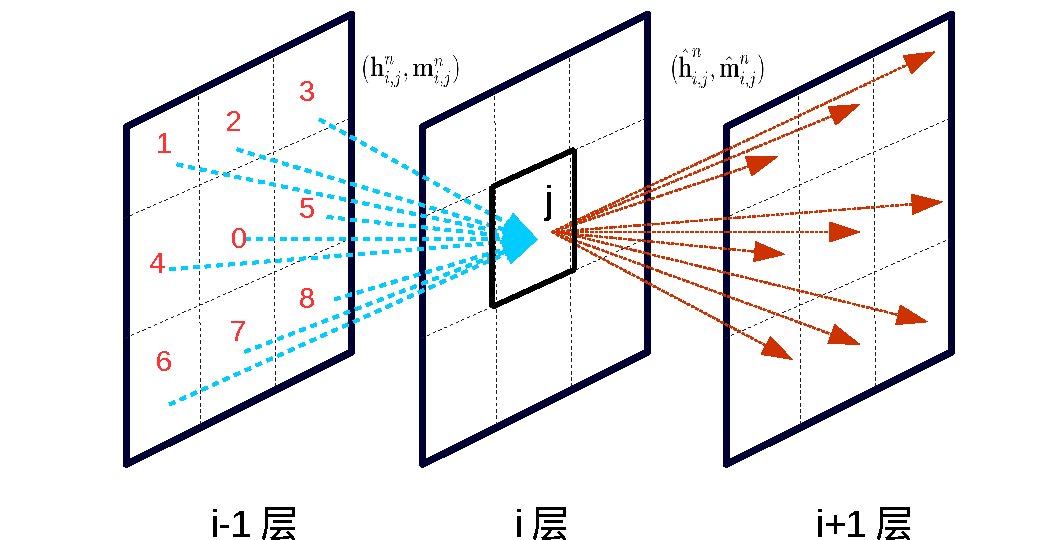
\includegraphics[width=\textwidth]{image/illustration/neighboring.pdf}
			\caption{九维网格型长短记忆网络层之间的通信示意图}
			\label{fig:neighboring}
		\end{figure}
		\end{column} 
		%%%%%%% new column
		\begin{column}{0.5\textwidth}
			\footnotesize
			\vspace{-1.5em}
			\begin{align}
				\begin{split}
				(\hat{\textbf{h}}_{i,j}^0,\hat{\textbf{m}}_{i,j}^0) &= \mbox{LSTM}(\textbf{H}_{i,j},\textbf{m}_{i,j}^0,\textbf{W}_i) \\
				(\hat{\textbf{h}}_{i,j}^1,\hat{\textbf{m}}_{i,j}^1) &= \mbox{LSTM}(\textbf{H}_{i,j},\textbf{m}_{i,j}^1,\textbf{W}_i) \\
				\vdots \\
				(\hat{\textbf{h}}_{i,j}^N,\hat{\textbf{m}}_{i,j}^N) &= \mbox{LSTM}(\textbf{H}_{i,j},\textbf{m}_{i,j}^N,\textbf{W}_i) \\
				\textbf{H}_{i,j} &= [\textbf{h}_{i,j}^0\mbox{ }\textbf{h}_{i,j}^1\mbox{ }...\mbox{ }\textbf{h}_{i,j}^N]^T
				\end{split}
			\end{align}
		\end{column}
    \end{columns}
	\footnotesize
	\vspace{-1em}
	\begin{block}{九维网格型长短记忆网络}
		\vspace{-0.7em}
		\begin{itemize}
			\item 每个位置的预测会受到上一层相邻八邻域特征的影响
			\item 随着层数的堆叠,每一位置将会有更大的感知域。
			\item 网格型长短记忆网络的层数通过实验来确定
		\end{itemize}
	\end{block}
}



\chapter{数据认证方案优化}
本章介绍对第二章提出的多节点联合数据认证机制进行的优化,利用多种方案提升数据认证机制的检测效率,降低节点能量消耗。
4.1节介绍无线传感网节点失效问题,提出了多路径抗节点失效的机制。
4.2节设计动态步长的多节点联合数据认证机制对传感网能量开销进行优化。
\section{多路径抗节点失效机制}
\subsection{数据认证中的节点失效问题}
由于无线传感网部署的环境恶劣,且容易受到攻击,使得节点的稳定性很难保证,整个网络的拓扑结构很容易发生变化。在3.3节中,我们讨论了在拓扑结构变化频率不大的情况下,通过传感器网络自身的维护机制,维护路径节点的上下行相关关系,适应无线传感网拓扑结构的变化。但是在节点失效或者被攻击比较频繁时,无线传感器网络结构变化很快,而原有的维护方案是通过重建路径来完成的,因而通信开销较大,造成大量节点能量损耗。

为了适应节点失效较多,传感网拓扑结构变化较大的情况,我们提出了多路径抗节点失效的方案。通过在初始化阶段预定义若干条不相交路径,对每个节点失效的情况预定义编织路径。但在一个传输阶段,只有一条路径被使用,并进行数据认证。当路径受到攻击,或者节点失效时,使用备用的不相交路径或者编织路径。通过多路径抗节点失效机制,提升了传输路径的稳定性,保证了路径中检测虚假数据报文的性能。

在多路径抗节点失效方案中,我们使用了单向hash链来分配密钥,提升了网络的安全性能,并节省了节点存储密钥的开销。每个节点使用单向hash函数从它的上行相关节点的密钥生成密钥,具体的密钥分配方案将在第五章进行详细描述。
\subsection{多路径抗节点失效机制设计实现}
在多路径抗节点失效机制中,节点上下行相关关系不是研究重点,不再详细介绍,沿用第三章中多跳长路径多节点联合数据认证的方案。我们在多路径抗节点失效机制中,使用了单向hash链来分配密钥,能更好地保证认证机制的安全性,降低节点保存密钥的存储开销。我们的路径抗节点失效机制包括了初始化和密钥分配、数据报文发送、路径中过滤、基站认证、路径选择五个阶段,如图~\ref{fig:MPA}所示:
\begin{figure}[htbp]
  \centering
  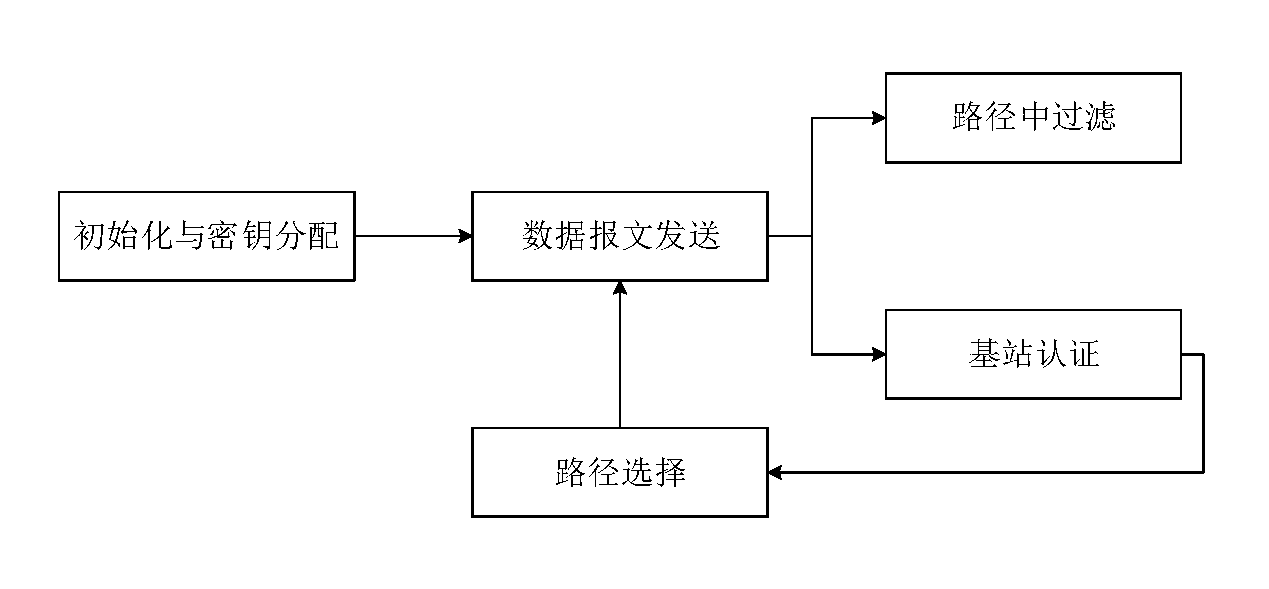
\includegraphics[width=5in]{MPA}
  \caption{多路径抗节点失效机制流程}
  \label{fig:MPA}
\end{figure}
\subsubsection{初始化和密钥分配}
传感器节点被部署到目标监测区域之后,基站会给每个节点生成一个共享密钥,这是每个节点与基站之间的共享密钥$AK_{si}$。然后每个簇通过预定的选举机制选举一个簇头节点,BS通过广播路由请求完成传感器网络的路由发现。

在多节点联合数据认证方案中,我们使用HELLO报文和ACK报文来完成路径发现和上下行相关关系的建立,在簇与BS之间建立一条多跳长路径。在多路径抗节点失效方案中,我们在初始化建立多条不相交长路径以及多条编织路径。虽然有多条路径,在我们的方案中,一次传输过程只会使用一条主路径,其他路径作为网络被攻击时的备选路径。

\begin{figure}[htbp]
  \centering
  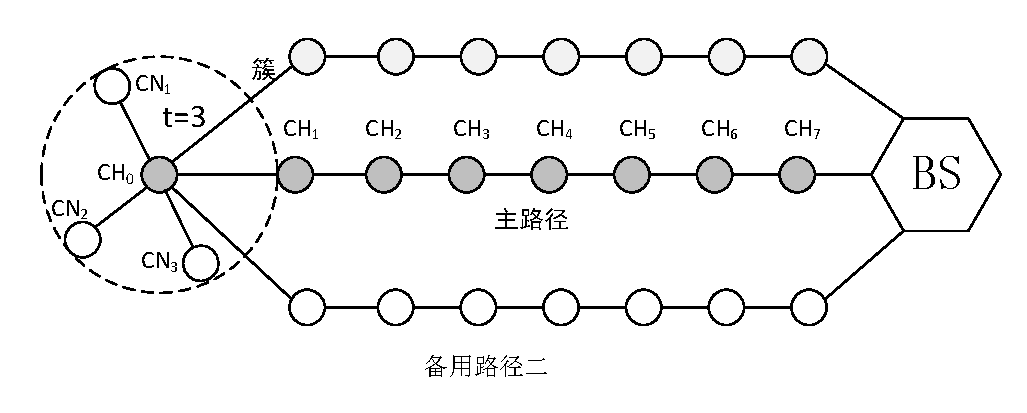
\includegraphics[width=5in]{IHAA1}
  \caption{多路径抗节点失效机制中的不相交路径}
  \label{fig:IHAA1}
\end{figure}
如图~\ref{fig:IHAA1}所示,簇与BS之间建立了3条不相交路径。不相交路径通过以下步骤建立:
\begin{compactitem}
  \item 建立一条簇头与BS之间的主路径。
  \item 建立一条与主路径不相交的,且跳数最短的路径,作为备用路径一。
  \item 建立一条与主路径以及备用路径一不相交的,且跳数最短的路径,作为备用路径二。
\end{compactitem}

\begin{figure}[htbp]
  \centering
  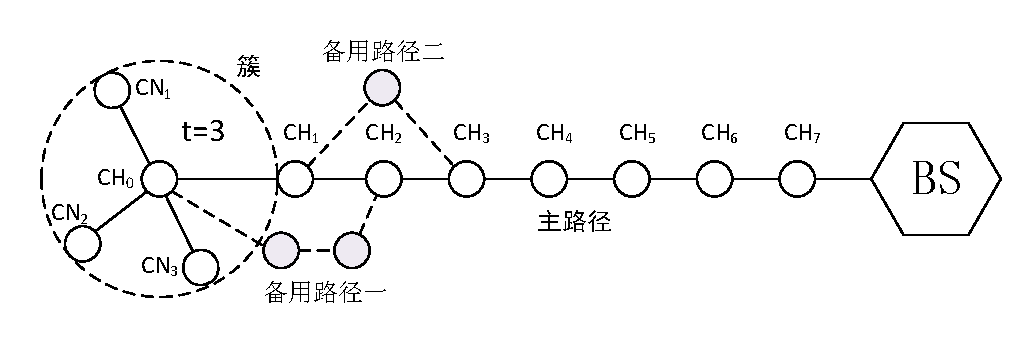
\includegraphics[width=5in]{IHAA2}
  \caption{多路径抗节点失效机制中的编织路径}
  \label{fig:IHAA2}
\end{figure}
如图~\ref{fig:IHAA2}所示,路径上的节点完成备用编织路径的建立。编织路径通过以下步骤建立:
\begin{compactitem}
  \item 建立一条簇头与BS之间的主路径。
  \item 对主路径上的每个节点,寻找不包括该节点的簇与BS之间的最短路径。在图~\ref{fig:IHAA2} 中,第一条编织路径就是不包括节点$CH_1$,从节点$CH_0$到节点$CH_2$之间的编织路径。相似的,第二条编织路径是不包括节点$CH_2$的从节点$CH_1$到节点$CH_3$的编织路径。
\end{compactitem}

\begin{figure}[htbp]
  \centering
  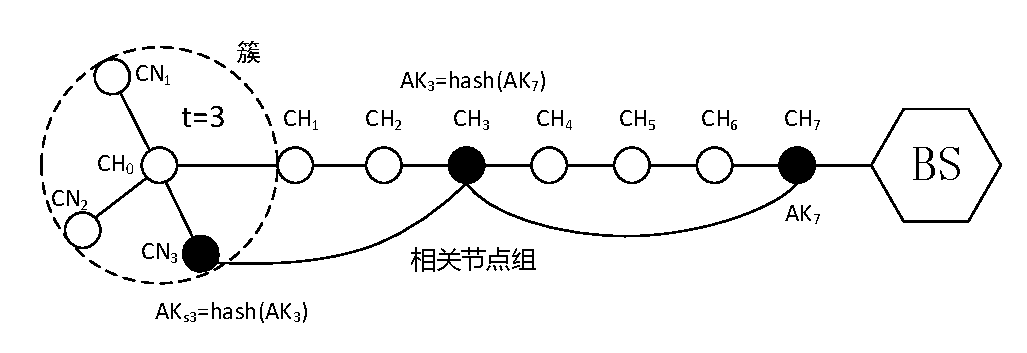
\includegraphics[width=5in]{IHAA3}
  \caption{多路径抗节点失效机制的密钥分配}
  \label{fig:IHAA3}
\end{figure}
在我们的多路径抗节点失效方案中,我们使用了单向hash链来进行密钥分配,如图~\ref{fig:IHAA3}所示。BS给每个上下行相关节点组生成一个$AK$,下行节点使用单向hash函数$H$从上行节点的密钥得到自己的密钥。图~\ref{fig:IHAA3}中所示,节点组\{$CN_3$,$CH_3$,$CH_7$\},距离BS最近的节点$CH_7$从BS获取BS生成的密钥$AK_7$,它的下行节点$CH_3$通过单向hash函数获取密钥$AK_3=H(AK_7)$。类似的,节点$CN_3$获取密钥$AK_{s3}=H(AK_3)$。通过这样的密钥分配,每个节点存储密钥的空间开销变小了,同时节点被攻击时丢失的密钥信息变少了。
\subsubsection{数据报文发送}
同多节点联合数据认证一样,簇节点监测到事件E以后,必须要$t+1$个节点都发出报文才能确认监测到的事件,如果没有至少$t+1$个节点的报文,则认为是无效事件。
簇节点MAC压缩后记作$XMAC(E)$:
\begin{equation}\label{XMAC}
\begin{split}
  XMAC(E)
  &=MAC(AK_{s1},E)\oplus MAC(AK_{s2},E)\oplus MAC(AK_{s3},E)\oplus MAC(AK_{s0},E)
\end{split}
\end{equation}
在多路径抗节点失效方案中,我们使用簇序号$C_i$来标记簇信息,代替原方案中的簇ID集,减小了传输开销。在簇头节点$CH_0$生成的报文R可以记作:
\begin{equation}\label{report1}
\begin{split}
  R=
  & E,C_i,h_0,XMAC(E),\{MAC(AK_{s1},E),\\
  & MAC(AK_{s2},E),MAC(AK_{s3},E),MAC(AK_0,E)\}
\end{split}
\end{equation}
\subsubsection{路径中过滤}
当节点$CH_i$从下行节点收到报文R以后,首先用相邻节点共享密钥对进行认证。然后使用其上下行相关节点的共享密钥对E计算MAC,并更新报文R。对于图~\ref{fig:IHAA3}中的节点$CH_3$,收到来自$CH_2$ 的报文后,首先使用单向hash函数计算得出其下行相关节点的密钥$AK_{s3}=H(AK_3)$。用$AK_{s3}$对事件$E$计算消息认证码$MAC(AK_{s3},E)$,与报文R中的第
$(h_0 - h_i)-((h_0 - h_i)/(t+1))\ast (t+1)=3$ 个相关节点MAC,也就是$MAC(AK_{s3},E)$进行比较,如果不同则丢弃报文R;如果相同则使用密钥$AK_3$ 对事件E计算消息认证码$MAC(AK_3,E)$,并替代原报文R中的$MAC(AK_{s3},E)$,将其转发给下一节点$CH_4$,更新后发送的报文R 为:
\begin{equation}\label{report2}
\begin{split}
  R=
  & E,C_i,h_0,XMAC(E),\{MAC(AK_1,E),\\
  & MAC(AK_2,E),MAC(AK_3,E),MAC(AK_0,E)\}
\end{split}
\end{equation}

\subsubsection{基站认证}
当BS收到报文R后,首先获取报文中的簇序号$C_i$,使用BS与簇$C_i$的节点ID列表中$t+1$个簇节点之间的共享密钥计算MAC,并用XOR 运算计算这$t+1$ 个MAC 的值,与报文R中的XMAC比较,如果不同,则丢弃报文。如果相同,则对事件E作出响应。
\subsubsection{路径选择}
当路径中节点受到攻击时,BS会收集到相应的信息,通过妥协节点检测技术\upcite{c4:mathews2007detecting},BS能确定哪些路径被攻击,妥协节点检测技术不是本文的重点,而是专注于妥协节点检测技术在数据认证中的应用。当BS确定了受攻击的路径以后,切换到未被攻击的备用路径。

同多节点联合数据认证机制中的节点关系维护相比,我们的多路径抗节点失效是通过预先定义备用路径,是一个应对节点攻击的前瞻性安全机制。而多节点联合数据认证机制中的节点维护是一种即时修复的方法,在节点失效或被攻击频率较高时,会造成传感器网络的传输路径不稳定,受攻击的影响更严重,还会造成大量的节点能量消耗。
\subsection{性能分析}
\subsubsection{安全性能分析}
在多跳长路径上多节点联合的数据认证机制中,被捕获节点的限度为$t$,当不少于$t$个节点被捕获,路径中的过滤就有可能无法检测出虚假数据报文。通过建立多跳备用路径和编织路径,多路径抗节点失效机制有更好的安全性能稳定性,在不少于$t$个节点被捕获时,仍能保证数据认证的安全性。

在多路径抗节点失效机制中,使用了基于单向hash链的密钥分配方案,保证了下行节点无法泄露上行节点的密钥。通过降低密钥信息丢失的概率,也提升了数据认证机会的安全性能。
\subsubsection{开销分析}
簇规模为$t+1$时,多路径的建立需要最少$N=(t+1)+d(t+1)$个节点,编织路径的建立需要至少$2(t+1)$个节点。
在提出的多路径抗节点失效机制中,MAC的计算是主要的计算开销,而且多路径抗节点失效机制中,每个节点进行认证前需要使用hash 函数进行密钥计算,使用SHA-1进行2byte的hash函数运算需要$1.52 \mu J$的能量开销。多路径抗节点失效机制需要维护多条备用路径和编织路径,有更高的能量开销,但是在虚假数据报文的比例较高时,因为其稳定的检测率,能明显减小传感网的能量开销。

\section{动态步长多节点联合数据认证}
\subsection{数据认证中的传输开销问题}
在无线传感网的多跳长路径传输中应用我们的多节点联合数据认证机制,能有效保证数据的安全传输,但是数据报文中附带了大量的MAC信息,加重了传感器节点的能量消耗。在规模化无线传感网中,由于传输路径跳数较多,数据传输实时性较高,节点的能量开销较大,因此安全机制的开销优化非常重要。

我们提出了一个动态步长的多节点联合数据认证,在传感器网络节点受攻击影响较小的时候,压缩所传输的报文,降低节点能量消耗,优化无线传感网的开销。
\subsection{动态步长多节点联合数据认证机制设计}
动态步长多节点联合数据认证是在多节点联合数据认证的基础上,对其进行改进,使得通信开销得到优化。
在4.1节中,我们讨论了在传感网拓扑结构变化较大时,使用多路径抗节点失效的机制来保证传感网传输稳定性。对于一条簇到BS之间的传输路径,如果路径比较稳定,则可以通过压缩数据报文的方式来降低传输开销。在我们提出的动态步长多节点联合数据认证机制中,是通过动态调整多节点联合认证中的节点组间隔步长来实现的。

在多节点联合数据认证中,根据步长的动态调整,对数据报文中的相关节点MAC进行相应程度的压缩处理,在路径传输的安全性与路径传输通信开销之间进行平衡,在保证路径安全性的情况下,降低通信开销。如图~\ref{fig:IHAA4}所示,是一个簇节点数为4,步长为3 的多节点联合数据认证。
\begin{figure}[htbp]
  \centering
  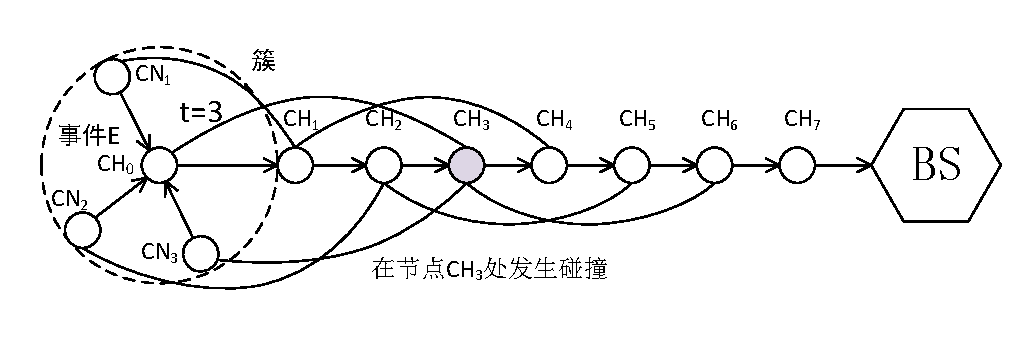
\includegraphics[width=5in]{IHAA4}
  \caption{动态步长多节点联合数据认证}
  \label{fig:IHAA4}
\end{figure}
\subsubsection{面向动态步长多节点联合数据认证的密钥分配}
%密钥分发,节点关系
在动态步长多节点联合数据认证中,我们也使用单向hash链来完成认证密钥的分配。不同于图~\ref{fig:IHAA3}中所示的密钥分配,在步长动态变化时,上下行相关节点组会发生碰撞,也就是不同的簇节点在同一个上下行相关节点组当中。如图~\ref{fig:IHAA4}中,节点$CH_0$和节点$CN_3$在同一个上下行相关节点组中,上行相关节点都是节点$CH_3$。

对于上下行相关节点的碰撞,我们通过对簇内节点添加虚拟的上下行顺序来解决。在如图~\ref{fig:IHAA4}的传输路径上,将4个簇节点的虚拟上下行关系设为$\{CN_3,CN_2,CN_1,CH_0\}$,也即步长为3时,节点$CH_0$是节点$CN_3$的上行相关节点。

\begin{figure}[htbp]
  \centering
  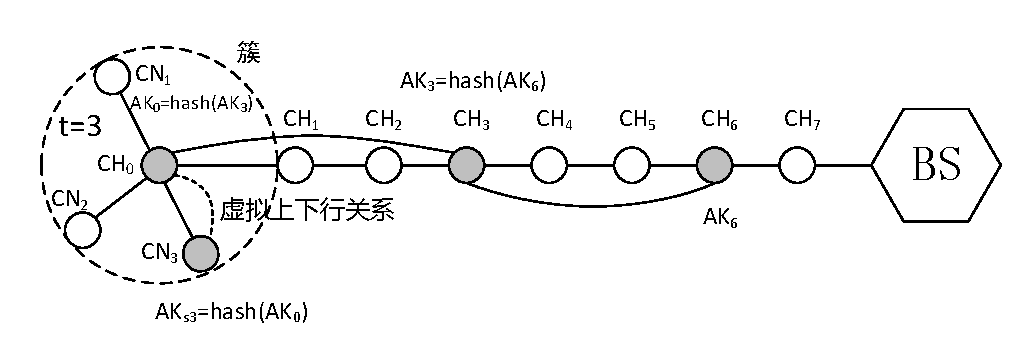
\includegraphics[width=5in]{IHAA5}
  \caption{面向动态步长多节点联合数据认证的密钥分配}
  \label{fig:IHAA5}
\end{figure}

如图~\ref{fig:IHAA5}所示,即为图~\ref{fig:IHAA4}所示的动态步长多节点联合数据认证情景的密钥传输示例。节点$CH_0$和节点$CN_3$都是簇节点,但是在同一个上下行相关节点组内,所以在节点$CH_0$和节点$CN_3$之间虚拟上下行相关关系,节点$CN_3$的密钥从节点$CH_0$的密钥计算而来,$AK_{s3}=H(AK_0)$。
\subsubsection{报文数据压缩传输}
使用单向hash链的密钥分配方案,给虚拟上下行相关节点分配了密钥以后,如图~\ref{fig:IHAA4}的动态步长多节点联合数据认证中,节点$CH_0$ 对簇节点数据进行整合之后的报文R可以表示为:
\begin{equation}\label{report3}
\begin{split}
  R=
  & E,C_i,h_0,XMAC(E),\{MAC(AK_{s1},E),MAC(AK_{s2},E),\\
  & MAC(AK_0,E)\oplus MAC(AK_{s3},E)\}
\end{split}
\end{equation}
其中$MAC(AK_0,E)\oplus MAC(AK_{s3},E)$为节点$CH_0$和节点$CN_3$的簇节点MAC使用XOR运算压缩后的结果。

我们用$p$表示步长,对于$h-h_0\leq p$的节点,在收到报文后,首先计算其下行相关节点的密钥。在图~\ref{fig:IHAA4}的示例中,节点$CH_3$ 收到报文R以后,首先计算下行相关节点的密钥$AK_0=H(AK_3)$。对事件E计算消息认证码$MAC(AK_0,E)$,并与报文R中第
$(h_0 - h_i)-((h_0 - h_i)/p)\ast p=3$个MAC进行比较,如果相同则用$MAC(AK_3,E)$替换之。如果不同则计算间隔一跳的下行相关节点的密钥$AK_{s3}=H(AK_0)$,对事件E计算消息认证码$MAC(AK_{s3},E)$,并与$MAC(AK_0,E)$进行XOR运算,
$MAC(AK_0,E)\oplus MAC(AK_{s3},E)$与报文R中第3个MAC进行比较,如果相同则用$MAC(AK_3,E)$替换之。
如果都不同,则表示是错误数据报文,但是不同于前面提出的方案,我们不将其直接丢弃,而是将$XMAC(E)$置为全0。
对于$h-h_0> p$的节点,同前述方案一样,只进行一次MAC验证。
在经过路径节点的验证后,节点将报文继续转发给上行节点。

\subsubsection{动态步长调整机制}
在BS收到报文以后,会对报文中的$XMAC(E)$进行验证。如果$XMAC(E)$为全0,则说明有错误数据报文在路径中被检测出来,这样说明传输路径的安全水平较低,则BS提高路径的传输步长$p$,这样能提升检测出错误数据报文的概率。如果BS连续收到若干个正常,达到一个阈值以后,我们认为路径是安全的,则BS降低路径的传输步长$p$,减小报文的大小,节约节点的传输能量。
\subsection{性能分析}
动态步长调整机制是建立在基站对路径的安全水平的评价基础上的,当路径的安全水平较高时,调整步长,压缩数据报文大小,降低传输的能量开销;当路径安全水平较低时,维持原有的步长,保证数据认证的安全性能。因此动态步长数据认证机制在安全性能上相比多节点联合数据认证无明显降低。

动态步长数据认证机制有效的在安全性能和能量开销之间进行权衡,在保证基本的安全性能的基础上优化能量开销。
在传感网中的虚假数据较少,也就是路径安全水平较高时,动态步长数据认证机制在能量开销上有明显的优化。

\section{本章小结}
本章针对多节点联合数据认证机制中,节点失效或者受攻击对路径中的节点相关关系的影响,我们提出了多路径抗节点失效的机制,设计实现了相关算法。为了优化多节点联合数据认证的通信开销,我们设计实现了动态步长多节点联合数据认证机制。对两个优化方案,都进行了相关安全性能的分析。




%%
% 结论
% 结论是毕业论文的总结,是整篇论文的归宿,应精炼、准确、完整。结论应着重阐述自己的创造性成果及其在本研究领域中的意义、作用,还可进一步提出需要讨论的问题和建议。
% modifyer: 黄俊杰(huangjj27, 349373001dc@gmail.com)
% update date: 2017-04-13
%%

\chapter{总结与展望}
\section{工作总结}
\section{研究展望}
\section{模板提供的命令}
冒号前面是命令,后面是显示的结果\\

pozhehao(破折号):\pozhehao \sysuspace mybold\{com\}(加粗斜体):\mybold{com} \sysuspace  etoday:\etoday\sysuspace ctoday:\ctoday\sysuspace


用于equation环境的命令

$norm :\norm{t}$

$argmax:\argmax{x}{y}\sysuspace argmin:\argmin{x}{y}$

$varmax:\varmax{x}{y}\sysuspace  varmin:\varmin{x}{y}$

$fncmax:\fncmax{x}{y}\sysuspace  fncmin:\fncmin{x}{y}$

$xxFnorm:\xxFnorm{x}\sysuspace xxFnormSqr:\xxFnormSqr{x}\sysuspace xxFprod:\xxFprod{x}{y}$

$xxOpVec:\xxOpVec{x}\sysuspace xxLprod:\xxLprod{x}{y}\sysuspace xxLprodVec:\xxLprodVec{x}{y}\sysuspace xxTensor:\xxTensor{x}$

$xxBracketY:\xxBracketY{x}\sysuspace xxBracketF:\xxBracketF{x}\sysuspace xxBracketH:\xxBracketH{x}$

\begin{figure}
	\centering
	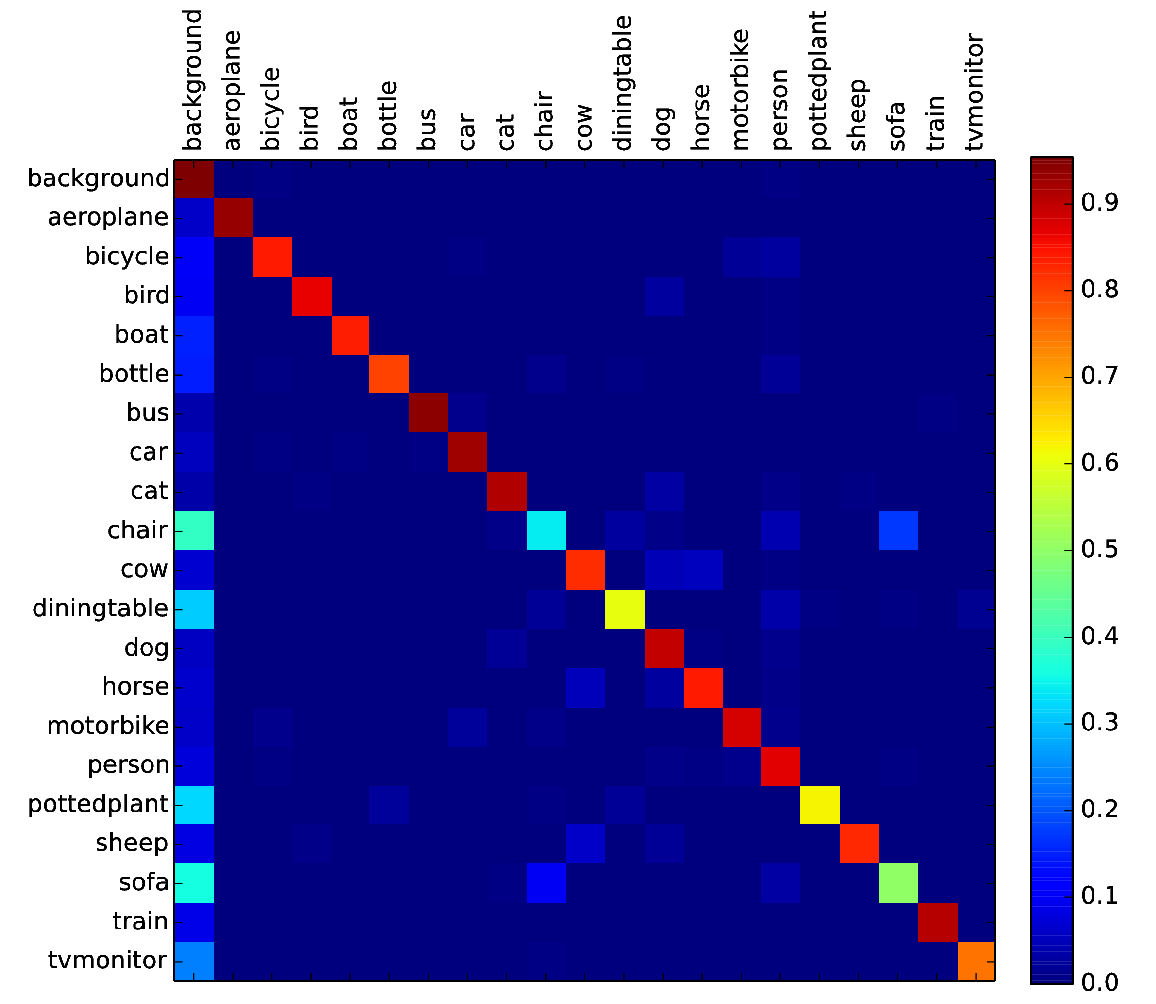
\includegraphics[width=0.5\textwidth]{image/result/confusion.pdf}
	\caption{镶嵌在文中的图像}
	\captionce[图注]{这是测试图注。}{A testing figure legend.}\label{fig:test}
	\label{fig:confusion}
\end{figure}
\section{致谢}
\subsection*{致谢}
\frame{
	\frametitle{致谢}
	\begin{block}{感谢每一个帮助过我的人}
	\begin{itemize}
		\item 首先要感谢的是我的指导老师的悉心指导
		\item 感谢师兄师姐、同学的帮助
		\item 感谢家人的支持
		\item 感谢答辩委员会的聆听和指导
	\end{itemize}
	\end{block}
	\vspace{-1em}
	\note{
		我的展示到此结束,我要感谢我的指导老师,师兄师姐同学,家人还有答辩委员会老师的聆听与指导。谢谢大家
	}
}
\frame{
	\frametitle{Q \& A}
	\begin{block}{Questions?}
	 ~\\ ~\\
	 \center{\Large{Thank you!}}
	 \\ ~\\ ~\\ ~\\ ~\\ 
	\end{block}
	\note{
		现在是问答时间。请问老师们对我的展示有什么疑问?
	}
}



\end{document}
